\documentclass{beamer}

\usepackage{listings}
\usepackage{tabulary}
\usepackage{amsmath}
\usepackage[utf8]{inputenc}
\usetheme{Madrid}
\setbeamersize{text margin left=0.1\textwidth,text margin right=0.1\textwidth}
\setbeamertemplate{section in toc}{\inserttocsection}
\lstset{language=python,
        keywordstyle=\color{red},
        basicstyle=\ttfamily,
        basicstyle=\small,
        frame = single,
        framexleftmargin=15pt,
        numbers=left,
        numberstyle=\small,
        numbersep=5pt,
        xleftmargin=0.05\textwidth,
        columns=fullflexible}
\definecolor{dgreen}{rgb}{0.,0.6,0.}
\definecolor{goldenrod}{rgb}{.9,0.6,0.1}

%Information to be included in the title page:
\title{Cross Validation}
\author{Cary Goltermann}
\institute{Galvanize}
\date{2016}

 \AtBeginSubsection[]
{
  \begin{frame}
    \frametitle{Overview}
    \tableofcontents[currentsection,currentsubsection]
  \end{frame}
}

\begin{document}

\frame{\titlepage}

\begin{frame}
  \frametitle{Overview}
  \tableofcontents[]
\end{frame}

\section{Cross Validation}
\subsection{Purpose}
\begin{frame}
  \frametitle{Purpose of Cross Validation}
  {\large There are two main reasons we use cross validation:} \vspace{4mm}
  \begin{enumerate}
    \item Find the best model to use. \pause
    \item Predict how well that model will perform on unseen data.
  \end{enumerate}
\end{frame}

\begin{frame}
  \frametitle{Modeling in an Equation}
  The problem that we are faced with when trying to create at predictive model coming up with a function that turns data into targets. Or in math:
  $$ y = f(X) + \epsilon $$

  where $\epsilon$ is error that our model doesn't account for. \vspace{2mm} 

  \pause
  \noindent\hfil\rule{\textwidth}{.4pt}\hfil \vspace{3mm}

  Eventually we will have many ways to make our $f$s and ways to format our data into different looking $X$s. Cross validation is the tool that we use to decide between all of these choices.
 
\end{frame}

\begin{frame}
  \frametitle{Comparing Linear Regressions}
  Imagine we have just a single variable $x_1$. We can create a linear regressions with different powers of this variable:

  $$ \hat{y}^{(1)} = \beta_0 + \beta_1 x_1 $$
  or
  $$ \hat{y}^{(2)} = \beta_0 + \beta_1 x_1 + \beta_2 x_1^2 $$
  or
  $$ \hat{y}^{(3)} = \beta_0 + \beta_1 x_1 + \beta_2 x_1^2 + \beta_2 x_1^3 + ... $$ \pause
  \begin{block}{Question}
    Which one of these equations has the most flexibility in describing a relationship between $x_1$ and $y$?
  \end{block}
\end{frame}

\begin{frame}
  \frametitle{Business Example}
  You are building a house-flipping company which will scrape Zillow for
  undervalued houses and buy them to flip. You're going to make money like this:

  $$ price_{future} = f(X) $$

  $$ Total\; expected = \sum_i price_{future,i} - price_{today,i} $$ 
  \pause

  \noindent\hfil\rule{\textwidth}{.4pt}\hfil \vspace{3mm}

  \centering
  What are the risks to your business scheme?
\end{frame}

\begin{frame}
  \frametitle{Linear Regression - How Do We Choose a Model?}
  \begin{itemize}
    \item Coefficients of linear regression minimize square error for given $X$.
    \item P-values are for the test of $H_0$: $\beta_i=0$.
    \item In assessing fit we have $\{R^2, AIC, BIC\} = f(X, \beta)$.
  \end{itemize}

  \noindent\hfil\rule{\textwidth}{.4pt}\hfil \vspace{3mm}
  \pause

  Which of these help us answer the question: "How will my model perform on data that it hasn't seen?" \vspace{2mm} \pause

  MSE is the only one that seems like it could be helpful here. Even then though, that measure is likely to be optimistic (Gauss-Markov Theorem).
\end{frame}

\subsection{Types of Fit}
\begin{frame}
  \frametitle{Types of Fit}
  \begin{columns}
    \column{1.2\textwidth}
    \begin{center}
      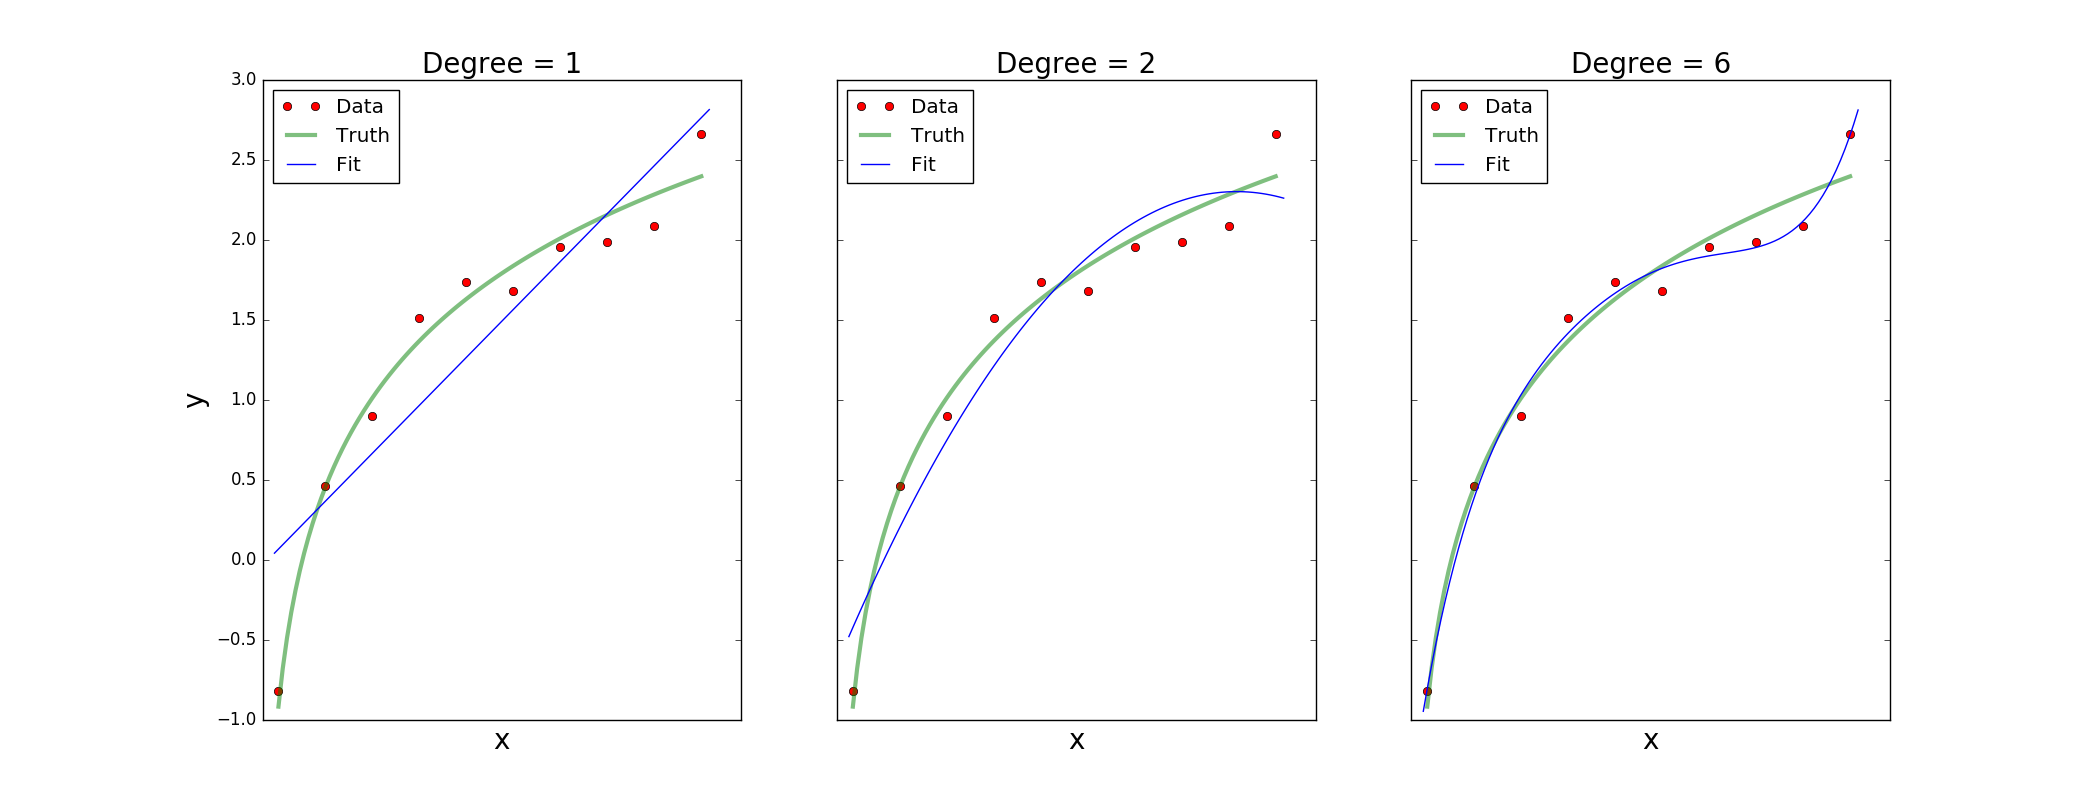
\includegraphics[width=\textwidth]{images/overfitting.png}
    \end{center}
  \end{columns} \pause

  \begin{block}{Question}
    Describe the fit of each model above.
  \end{block}
\end{frame}

\begin{frame}
  \frametitle{Types of Fit}
  \begin{columns}
    \column{1.2\textwidth}
    \begin{center}
      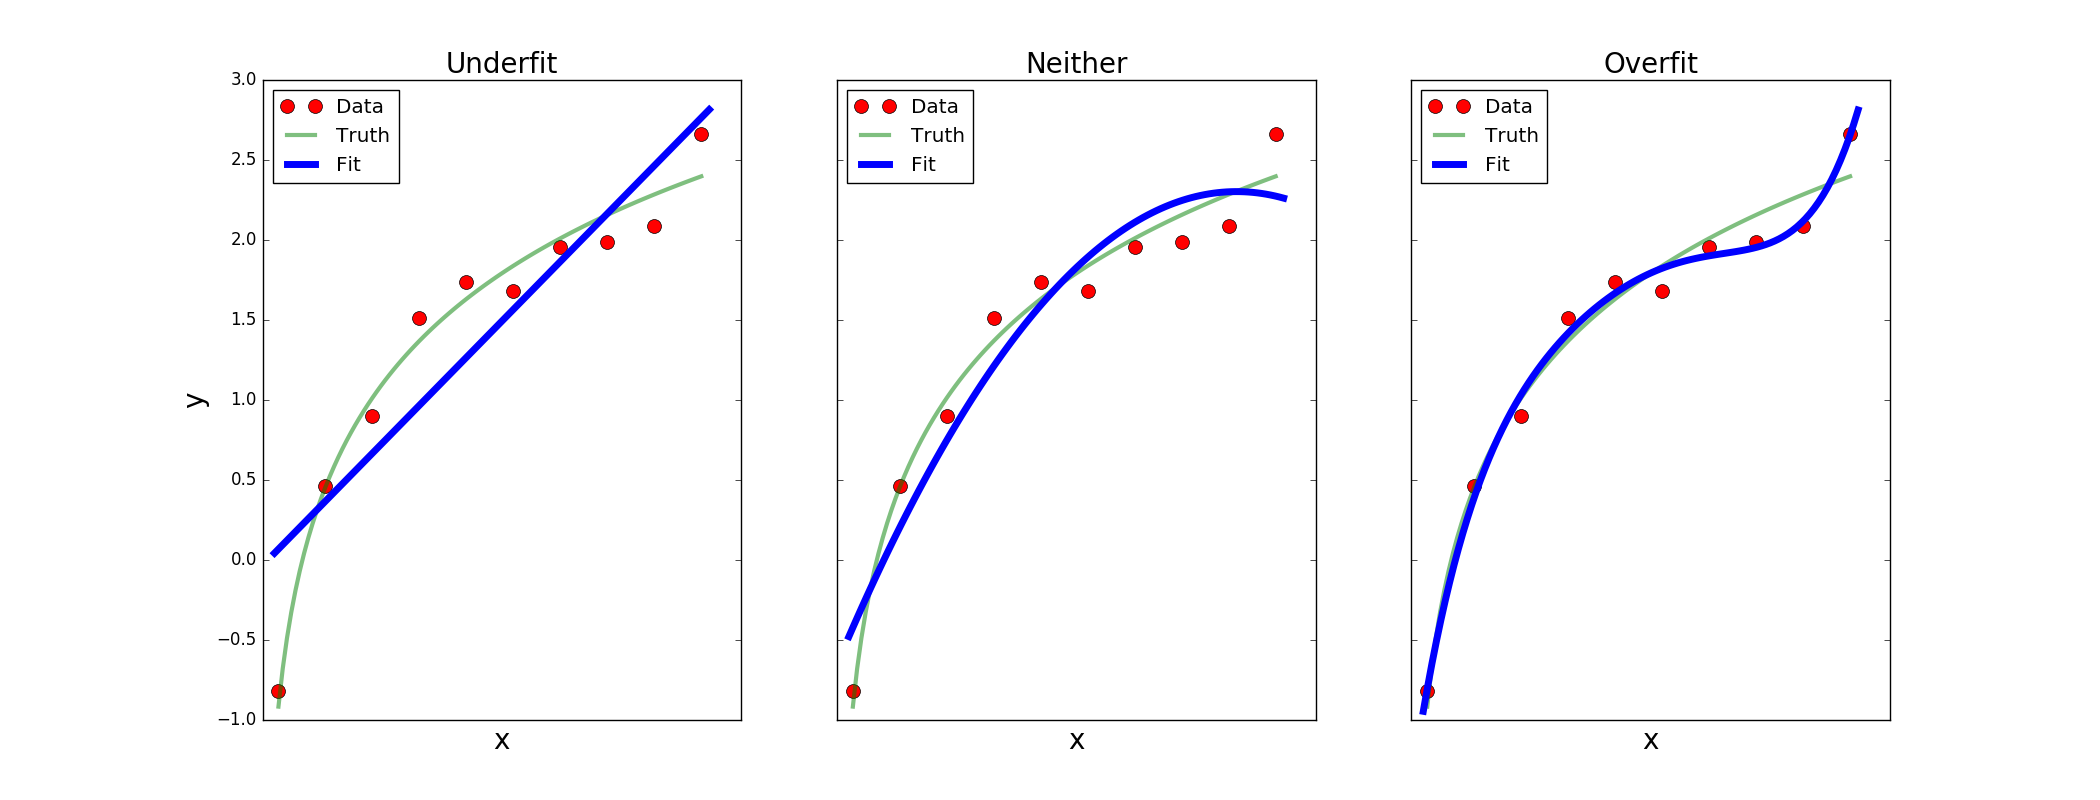
\includegraphics[width=\textwidth]{images/overfitting_labeled.png}
    \end{center}
  \end{columns}

  \begin{block}{Question}
    What is (potentially) wrong with each of these models?
  \end{block}
\end{frame}

\begin{frame}
  \frametitle{Over and Underfitting}
  Both of these problems with fit come down to a failure of  the true relationship between $y$ and $X$. \vspace{3mm} \pause

  {\large \textcolor{blue}{Underfitting}}
  \begin{itemize}
    \item Model does not fully capture the signal in $X$.
    \item Model is not flexible enough.
  \end{itemize} \vspace{3mm} \pause

  {\large \textcolor{blue}{Overfitting}}
  \begin{itemize}
    \item Model attributes to signal that which is truly noise.
    \item Model is too flexible.
  \end{itemize}
\end{frame}

\subsection{Kinds of Model Error}
\begin{frame}
  \frametitle{Bias and Variance}
  Typically we refer to the error caused by under and overfitting by their statistical names: \textbf{\textcolor{blue}{bias}} and \textbf{\textcolor{blue}{variance}}. \vspace{4mm} \pause

  One important thing to note is that together bias and variance make up all \textbf{reducible} sources of error in a model. \vspace{2mm} \pause

  \begin{align*}
    y &= f(X) + \epsilon \\
    \hat{y} &= \hat{f}(X) \\
    E[(y - \hat{f}(x))^2] &= Var(\hat{f}(x)) + Bias^2(\hat{f}(x)) + Var(\epsilon)
  \end{align*}
  $$ \textcolor{blue}{Bias(\hat{f}(x))} = E[\hat{f}(x) - f(x)] \qquad \textcolor{blue}{Var(\hat{f}(x))} = E[\hat{f}(x)^2] - E[\hat{f}(x)]^2 $$
\end{frame}

\begin{frame}
  \frametitle{Bias-Variance Graphically}
  \begin{columns}
    \column{1.2\textwidth}
    \begin{center}
      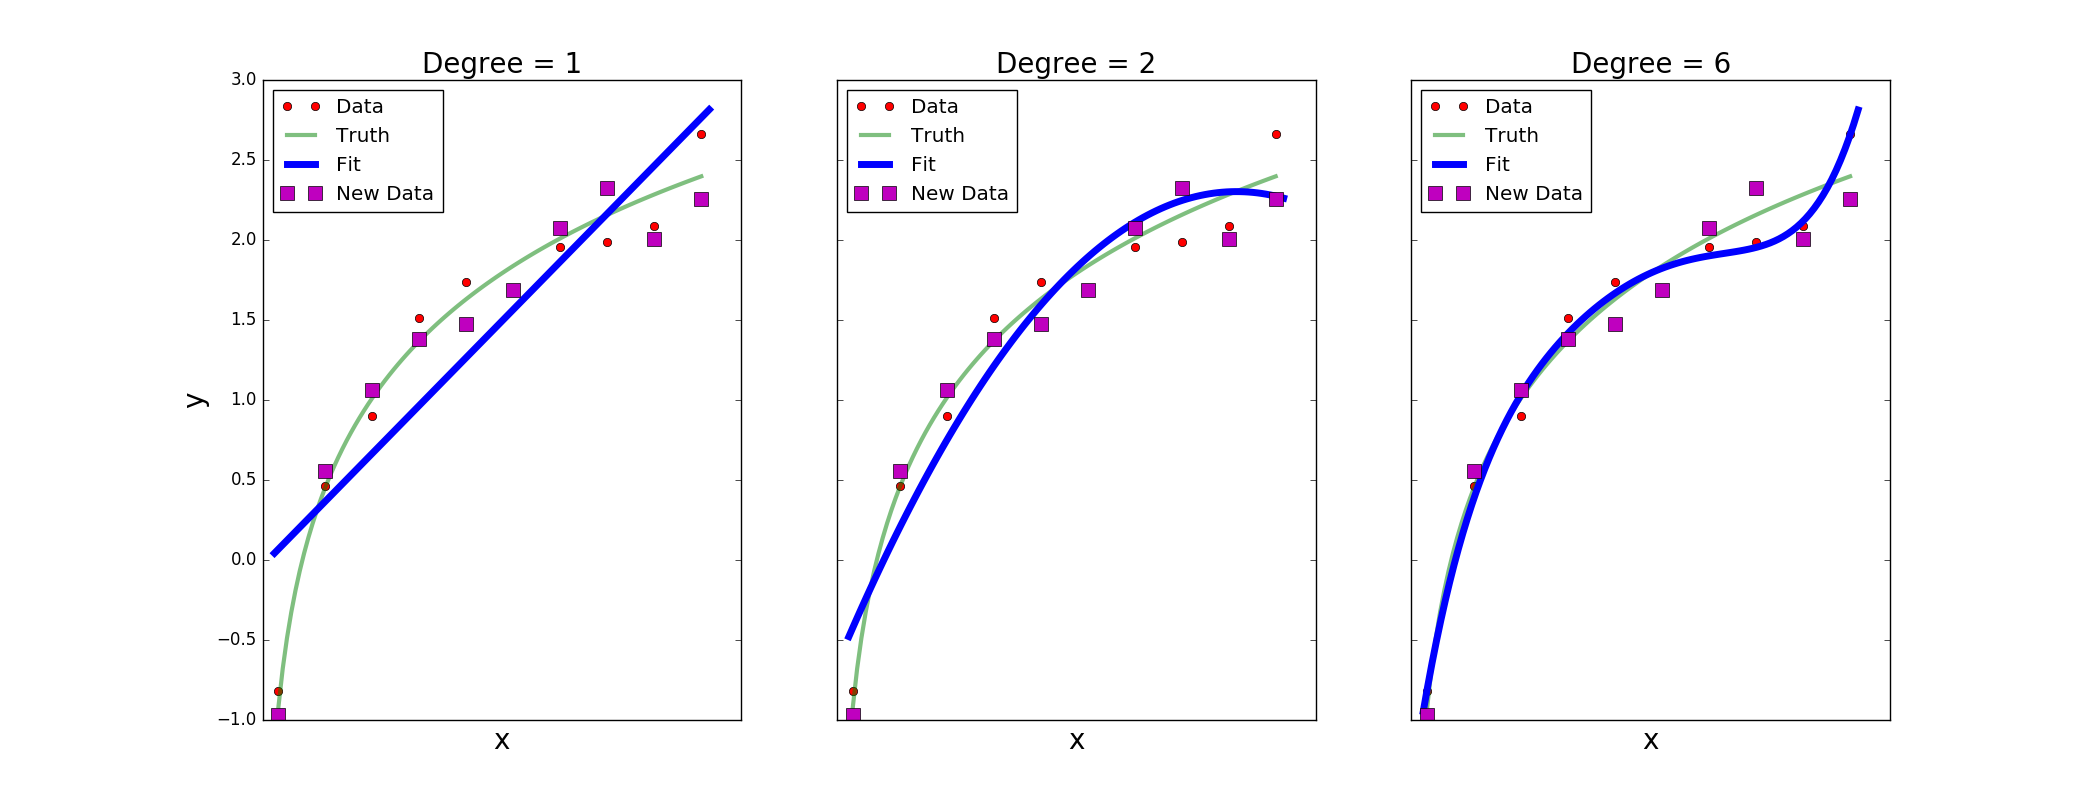
\includegraphics[width=\textwidth]{images/overfitting_new_data.png}
    \end{center}
  \end{columns}
\end{frame}

\subsection{Model Selection}
\begin{frame}
  \frametitle{Training/Validation Split}
  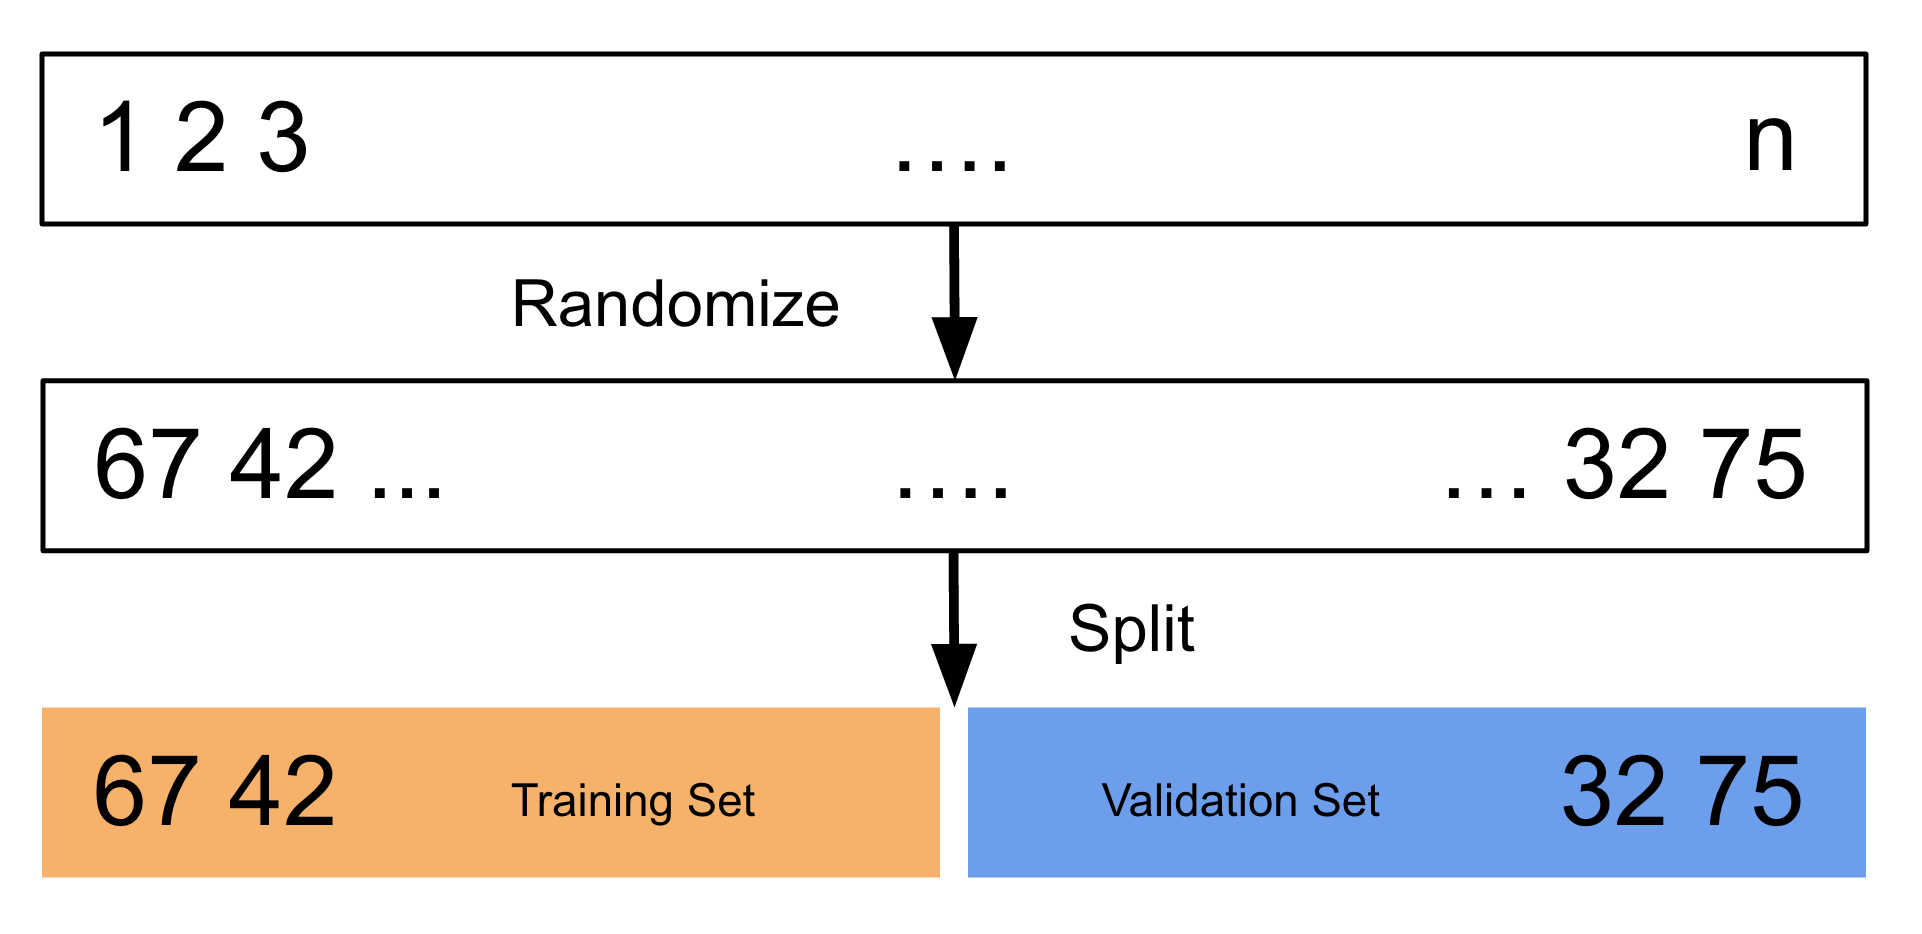
\includegraphics[width=\textwidth]{images/train_validation_split.png}
\end{frame}

\begin{frame}
  \frametitle{Procedure}
  \begin{enumerate}
    \item Split into training/validation sets.
    \item Use training set to train several model of varying complexity.
    \item Evaluate each model using the validation set.
    \item Keep the model that performs best over in validation.
  \end{enumerate}
\end{frame}

\begin{frame}
  \frametitle{How to Use}
  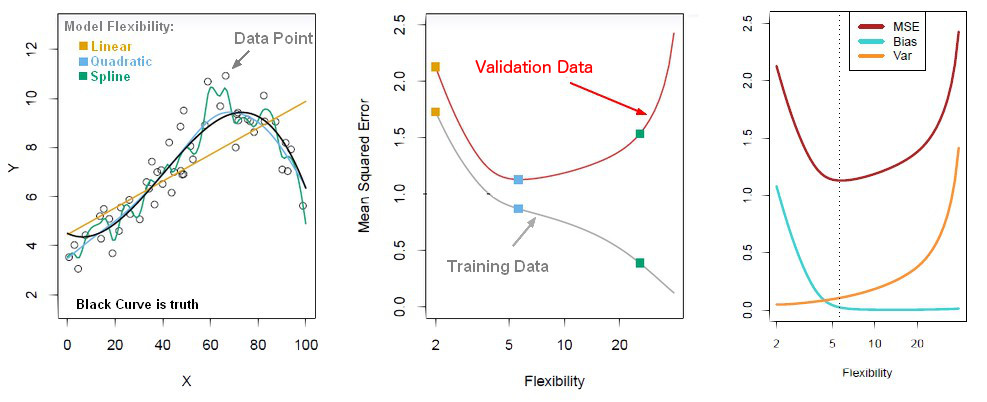
\includegraphics[width=\textwidth]{images/bias_variance_tradeoff.jpg}
\end{frame}

\begin{frame}
  \frametitle{Train Test Errors}
  \begin{center}
    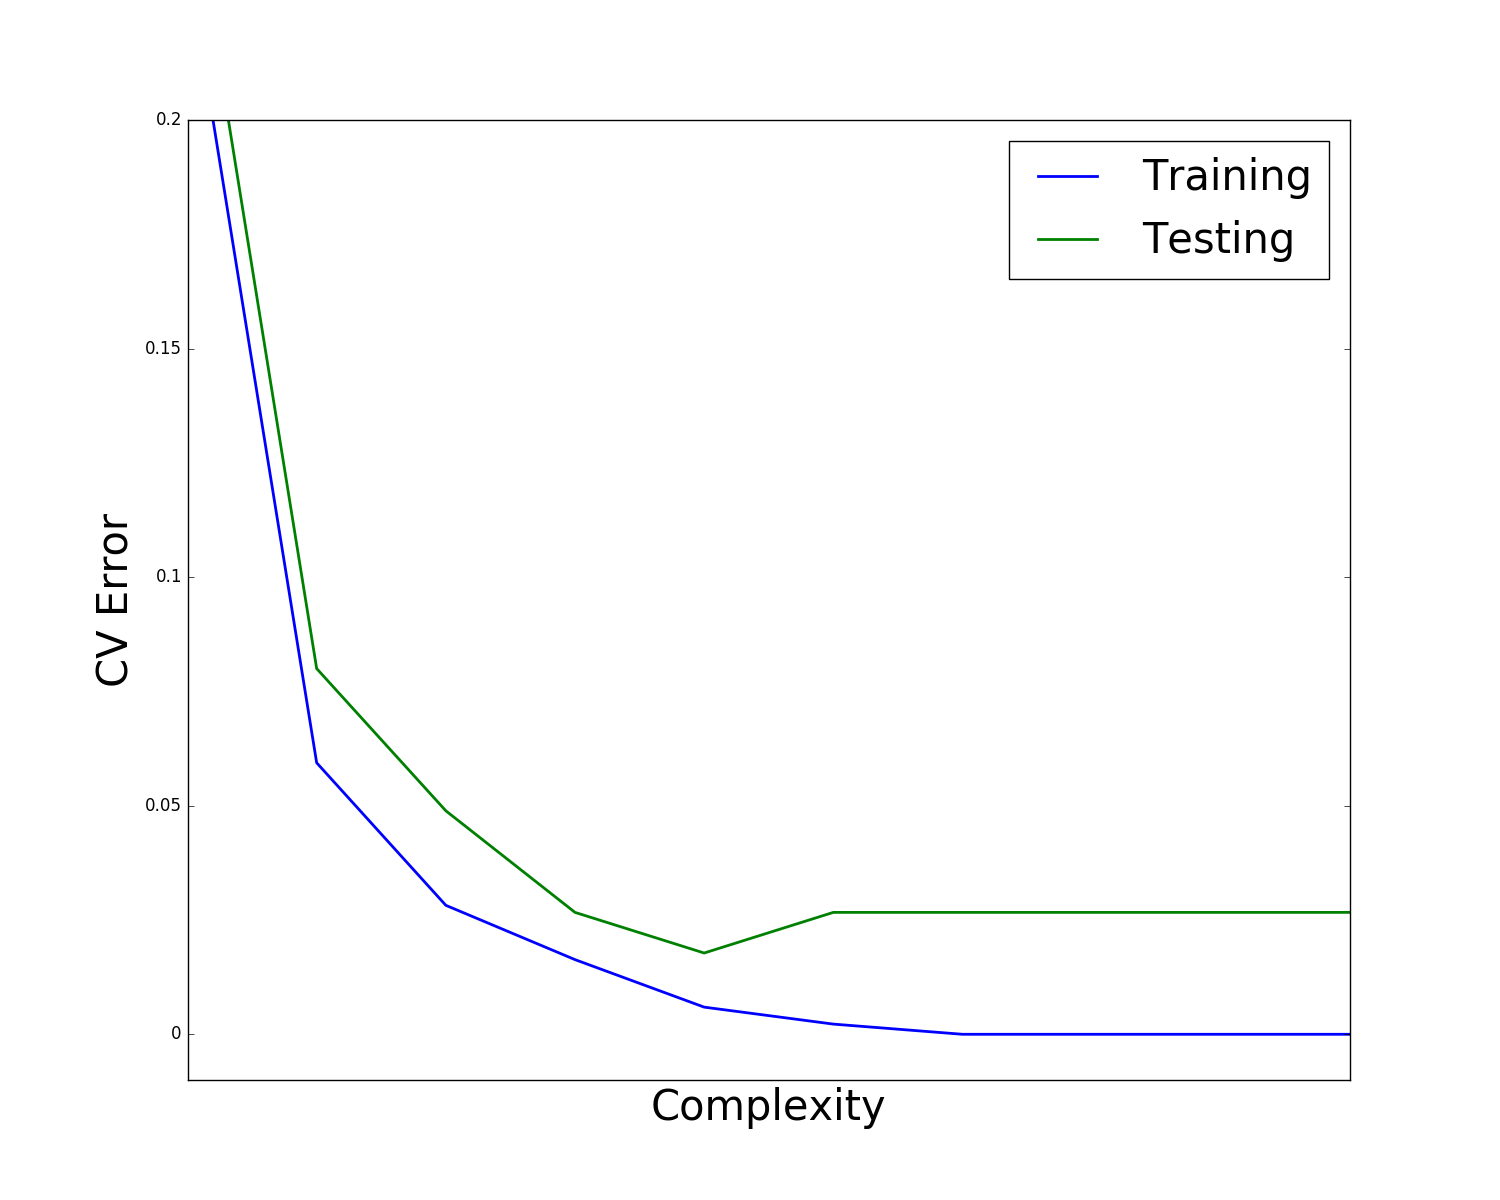
\includegraphics[width=0.9\textwidth]{images/train_test_error.png}
  \end{center}
\end{frame}

\begin{frame}
  \frametitle{Discussion}
  \begin{block}{Question}
    Given the train-validation split procedure just described, why might we doubt that our chosen model is truly the best?
  \end{block} \vspace{4mm} \pause
  \textit{Hint: what if we're ``unlucky''?}
\end{frame}

\subsection{K-Fold Cross Validation}
\begin{frame}
  \frametitle{K-Fold Cross Validation}
  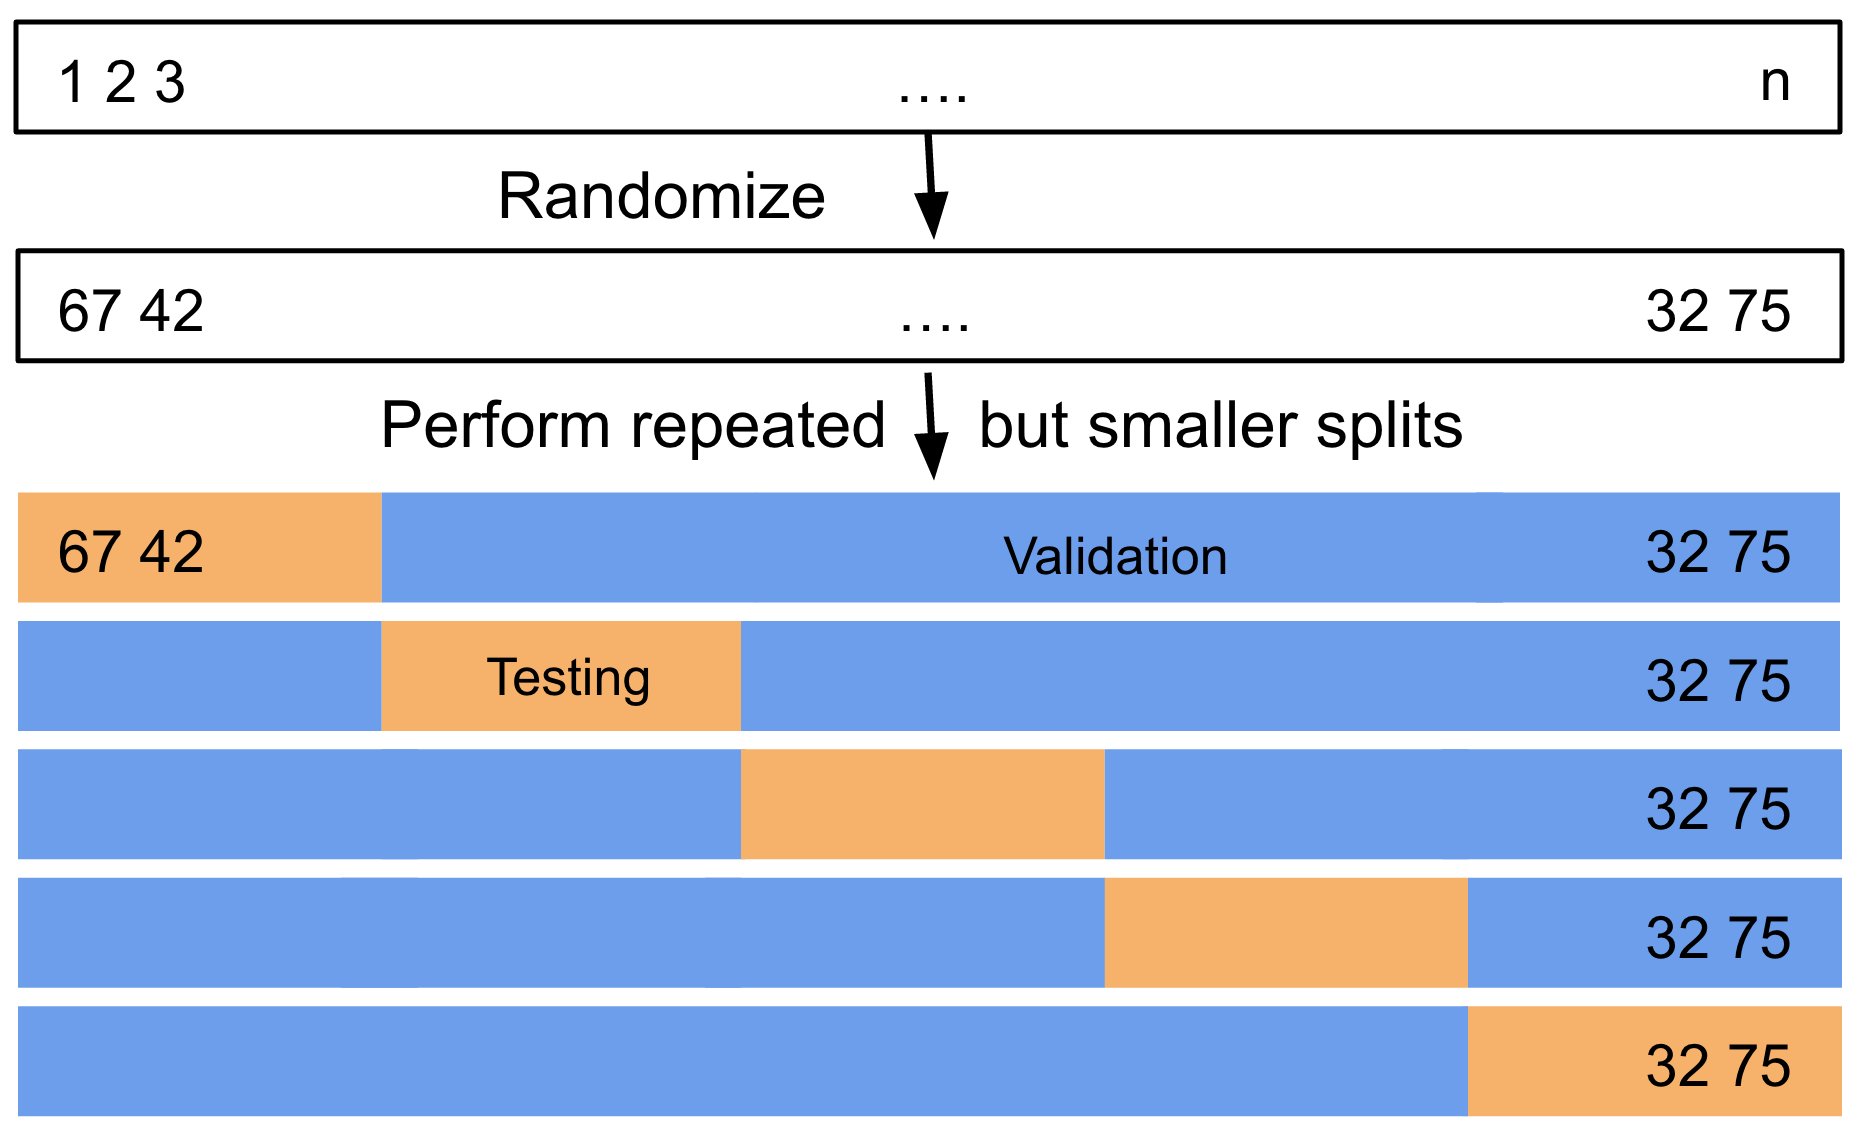
\includegraphics[width=\textwidth]{images/k_fold_split.png}
\end{frame}

\begin{frame}
  \frametitle{K-Fold Example, $K=3$}
  Given a dataset $D$,
  \begin{enumerate}
    \item For each candidate model:
    \begin{enumerate}
      \item Partition $D$ into 3 parts, $D_1$, $D_2$, $D_3$.
      \item For each $D_i$:
        \begin{enumerate}
          \item Mark $D_i$ as the validation set.
          \item Mark the remaining $D_{j \ne i}$ as the training set.
          \item Train candidate models on the training set.
          \item Append the model errors to a list.
        \end{enumerate}
      \item Compute the mean errors for each of the model error lists created in the last step.
    \end{enumerate}
    \item Select the model with the lowest mean error.
    \item Retrain the model on entire dataset, $D$.
  \end{enumerate}
\end{frame}

\begin{frame}
  \frametitle{How Good is K-Fold CV?}
  \begin{block}{Question}
    How comparable is the error metric we get from K-Fold CV error we can expect on unseen data?
  \end{block} \vspace{4mm} \pause
  \textit{Hint: In train-validation split, what happened when our validation set wasn't representative of unseen data?}
\end{frame}

\begin{frame}
  \frametitle{Train-Validation-Test}
  Just as the errors observed in training are conservative because those errors apply to the data that the model had the opportunity to learn from during training. \vspace{6mm}

  Similarly, the errors observed in cross validation are conservative because those errors are realized on data that the model selection process got to see during training. \vspace{1mm}

  \noindent\hfil\rule{\textwidth}{.4pt}\hfil \vspace{3mm}
  \pause
  
  How, then, do we get a good idea on how our model will perform "in the wild"?
\end{frame}


\begin{frame}
  \frametitle{Cross Validation Workflow}
  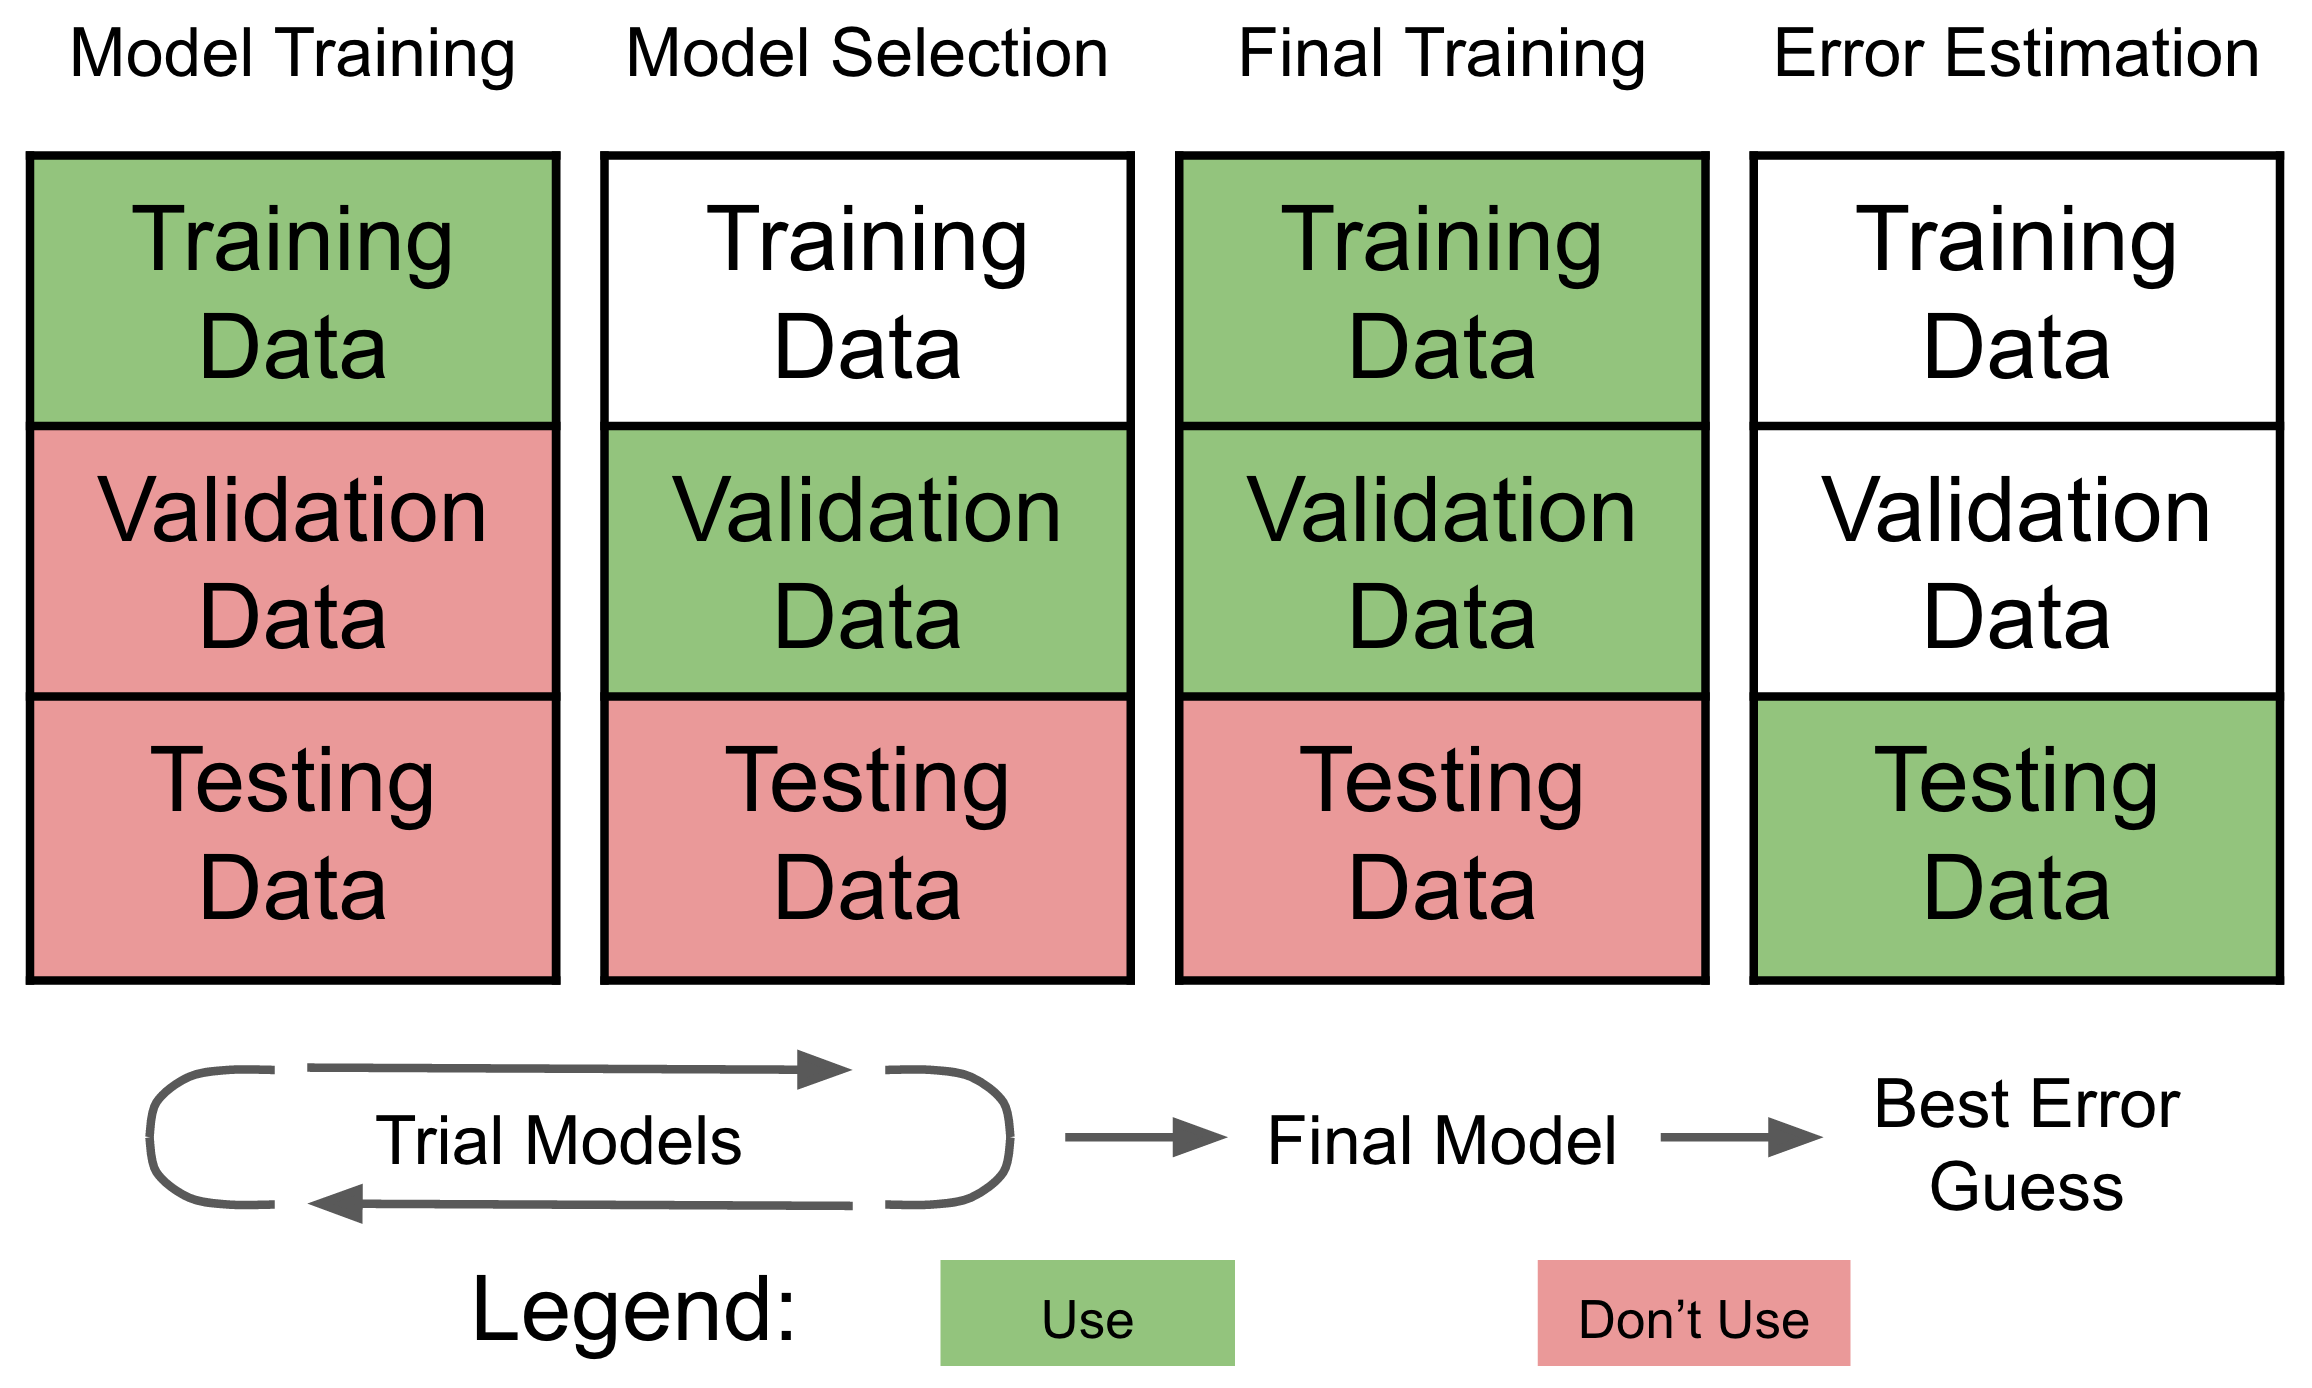
\includegraphics[width=\textwidth]{images/cv_workflow.png}
\end{frame}

\begin{frame}
  \frametitle{Other CV Techniques}
  \begin{tabulary}{\textwidth}{LL}
    \textcolor{blue}{Leave One Out CV} & Like K-Fold, except we set $k=n$. \\ [2mm]
    \textcolor{blue}{Stratified K-Fold} & Like K-Fold, except proportion of subgroups is maintained within each fold. \\ [2mm]
    \textcolor{blue}{Time-Series CV} & Never train on data from the future. \\ [2mm]
  \end{tabulary}
\end{frame}

\end{document}
